% !TEX root = ../lab1_report.tex
% ==========================================================
% 实验四：发动机虚拟流动实验
% ==========================================================
\section{实验四：发动机虚拟流动实验}

\subsection{实验目的}

掌握气流在发动机内部运动的特点及变化规律。

\subsection{实验装置}

气流经过某发动机内部流动的视频文件，展示气流在发动机各主要部件中的流动状态，包括压气机流动（正常与失速）、燃烧室流动、涡轮流动、排气混合器和加力燃烧室流动。

\subsection{实验步骤及内容}

\subsubsection{压气机流动观察}

观察气流经过压气机时流道和气流状态的变化，尤其注意正常流动和失速的差别。

\begin{figure}[H]
    \centering
    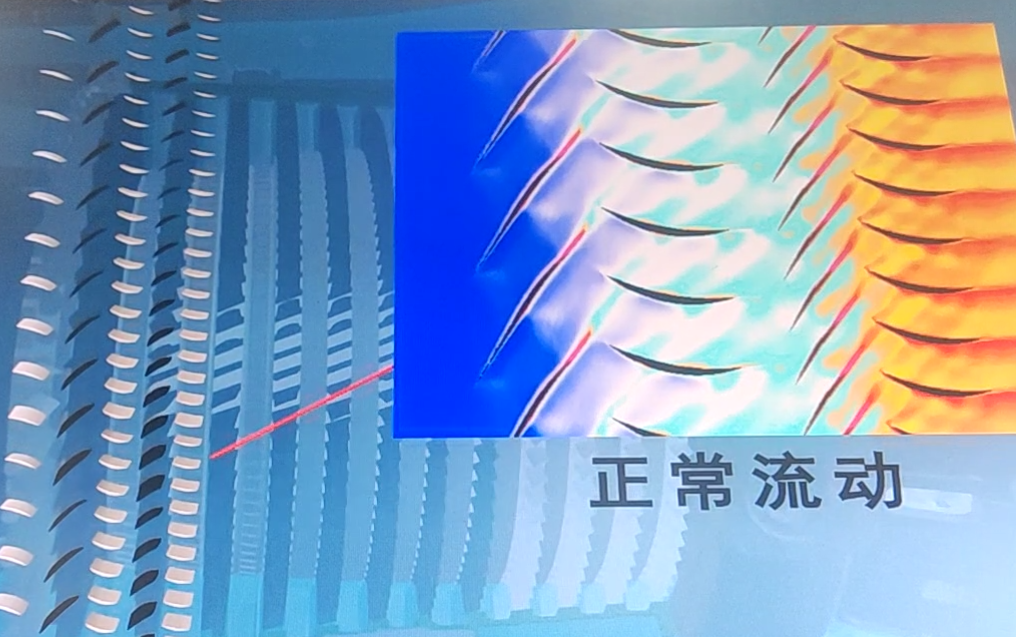
\includegraphics[width=0.90\textwidth]{figures/图4.png}
    \caption{压气机叶栅正常流动——设计攻角下气流顺畅通过叶栅通道}
    \label{fig:comp_normal}
\end{figure}

\textbf{正常工况（图~\ref{fig:comp_normal}）：} 在设计冲角下，气流顺畅地流过压气机叶栅通道，附面层（边界层）紧贴叶片吸力面与压力面，未发生明显的流动分离。通道内存在连续且均匀的逆压梯度，实现气流动能向压力能的有效转化。各叶片通道内流场均匀一致。

\begin{figure}[H]
    \centering
    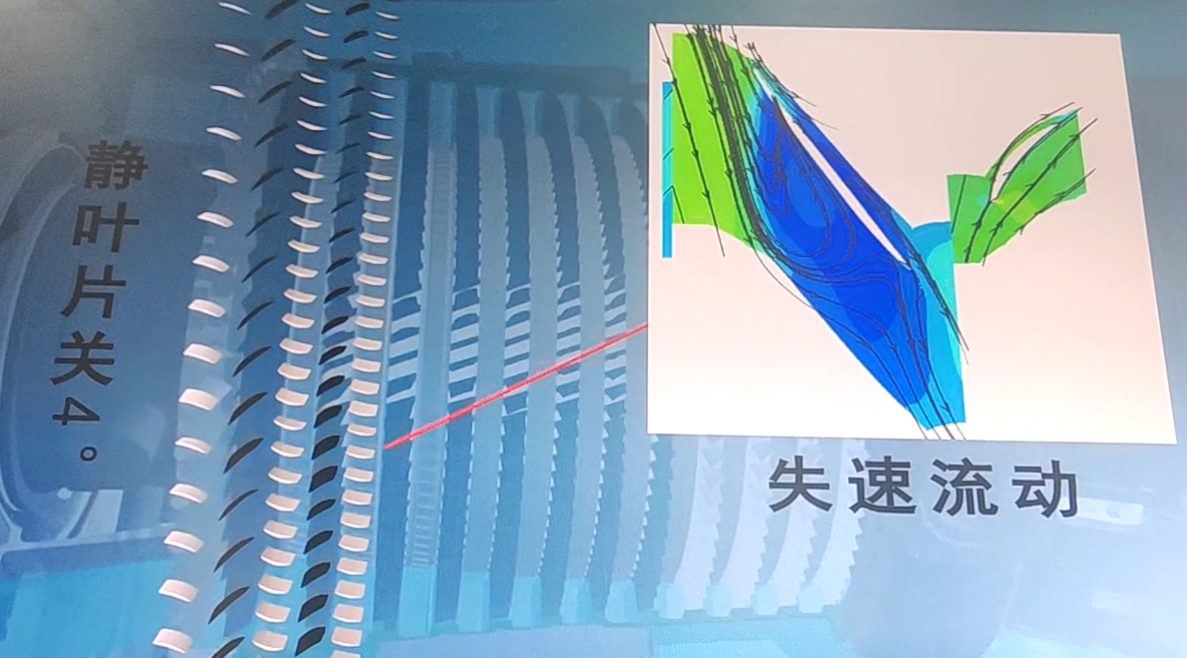
\includegraphics[width=0.90\textwidth]{figures/图5.png}
    \caption{压气机失速工况——关4°时吸力面出现大面积分离}
    \label{fig:comp_stall}
\end{figure}

\textbf{失速工况（图~\ref{fig:comp_stall}）：} 当静叶片角度异常（图中标注为关4°），导致气流冲角过大时，在叶片吸力面观察到严重的附面层分离。分离区（深蓝色区域）产生了巨大的旋涡和回流，形成了强烈的气动阻塞（Blockage）。这使得压气机该级通道丧失了正常的增压能力，是诱发发动机喘振的直接原因。

\subsubsection{燃烧室流动观察}

观察气流经过燃烧室时的流动情况，尤其注意内部的涡系结构和温度分布。

\begin{figure}[H]
    \centering
    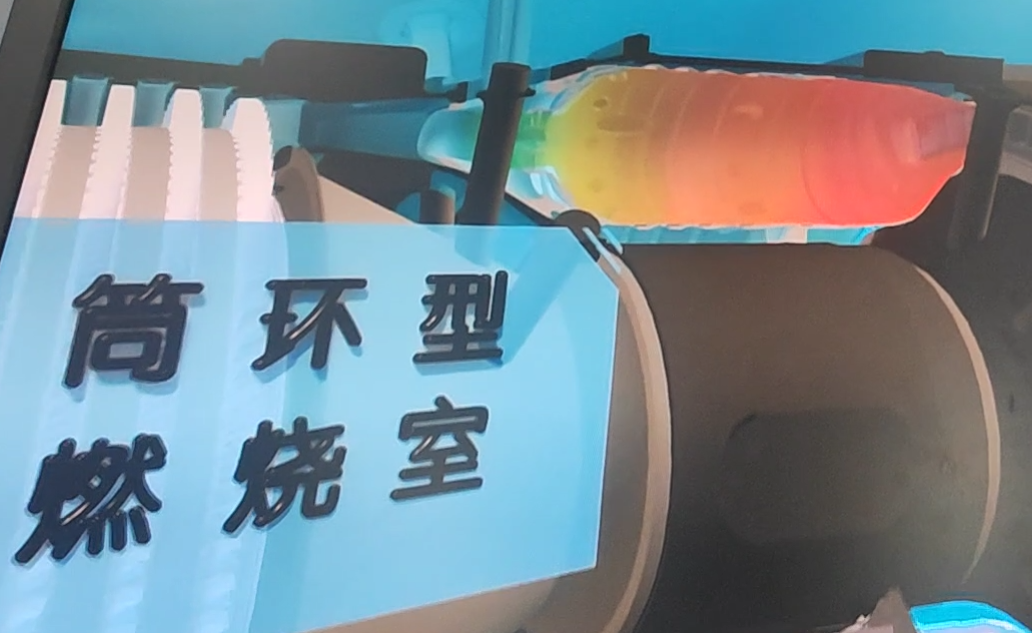
\includegraphics[width=0.85\textwidth]{figures/图6.png}
    \caption{燃烧室结构剖面}
    \label{fig:comb_struct}
\end{figure}

\begin{figure}[H]
    \centering
    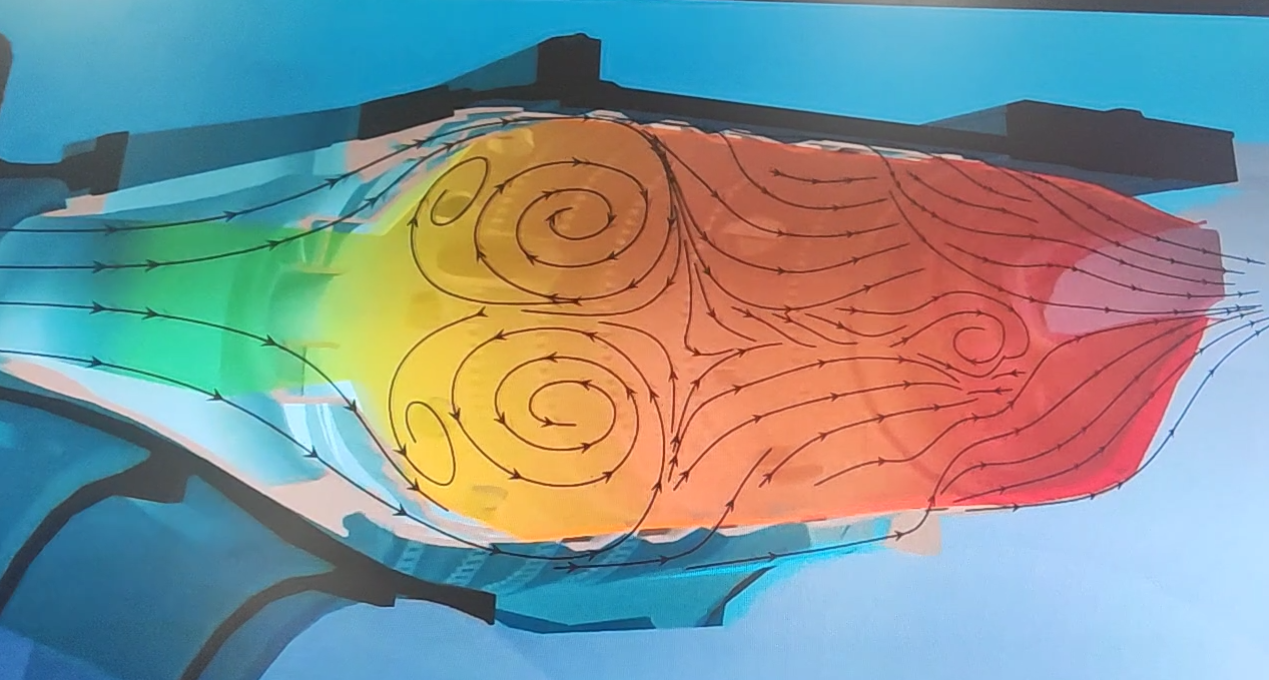
\includegraphics[width=0.90\textwidth]{figures/图7.png}
    \caption{主燃烧室流场——头部双涡回流区}
    \label{fig:comb_flow}
\end{figure}

\textbf{流场拓扑（图~\ref{fig:comb_flow}）：} 通过二维流线切面清晰观察到，主燃区前段形成了对称的双涡回流区。这是由于头部旋流器的强旋流作用所产生的中心驻点反向流动。这个回流区大幅降低了局部气流的轴向速度，使得燃油微滴有充足的时间蒸发并与空气混合，同时将燃烧后的高温燃气带回根部点燃新鲜混气——这是维持核心机连续稳定燃烧的关键气动结构。

\begin{figure}[H]
    \centering
    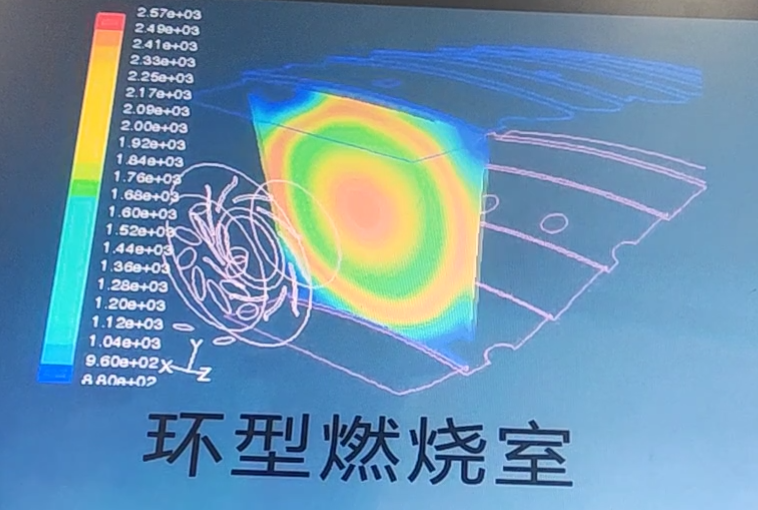
\includegraphics[width=0.90\textwidth]{figures/图8.png}
    \caption{燃烧室温度云图——中心高温区与壁面冷却}
    \label{fig:comb_temp}
\end{figure}

\textbf{温度分布（图~\ref{fig:comb_temp}）：} 温度云图印证了燃烧室截面中心呈现极高的温度梯度。壁面冷却气膜将火焰筒壁面与高温燃气（可达 2000\textasciitilde2400 K）隔离，保证火焰筒结构完整性。

\subsubsection{涡轮流动观察}

\begin{figure}[H]
    \centering
    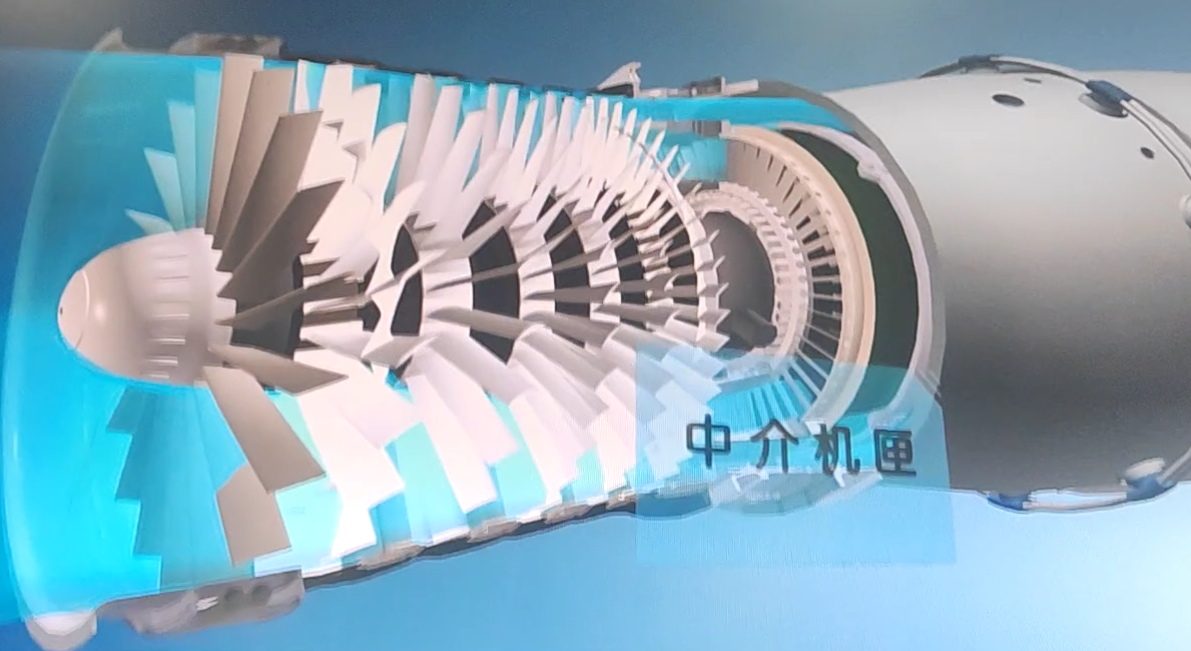
\includegraphics[width=0.85\textwidth]{figures/图1.png}
    \caption{发动机整体结构示意}
    \label{fig:engine_overview}
\end{figure}

\begin{figure}[H]
    \centering
    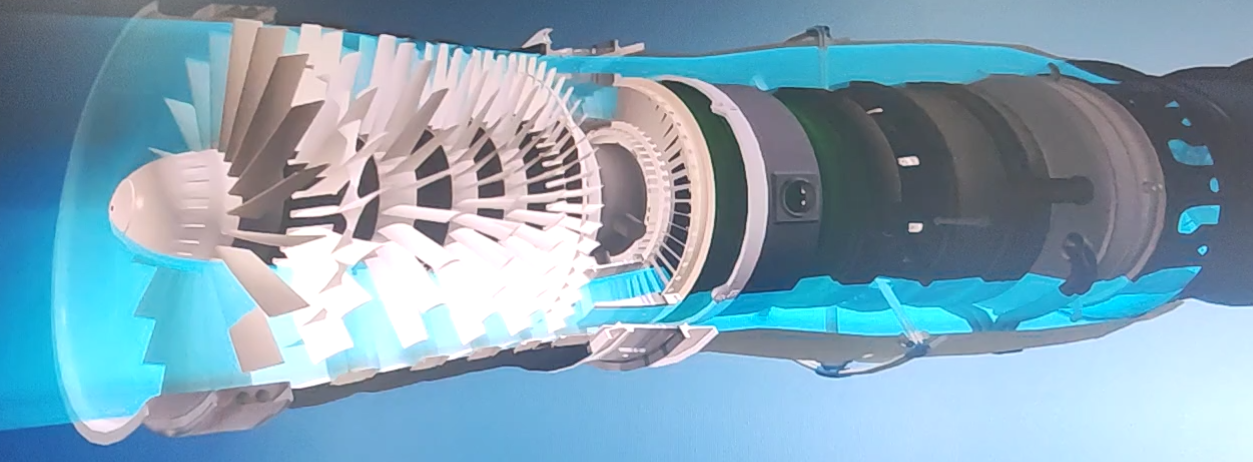
\includegraphics[width=0.85\textwidth]{figures/图2.png}
    \caption{发动机剖面结构}
    \label{fig:engine_section}
\end{figure}

\begin{figure}[H]
    \centering
    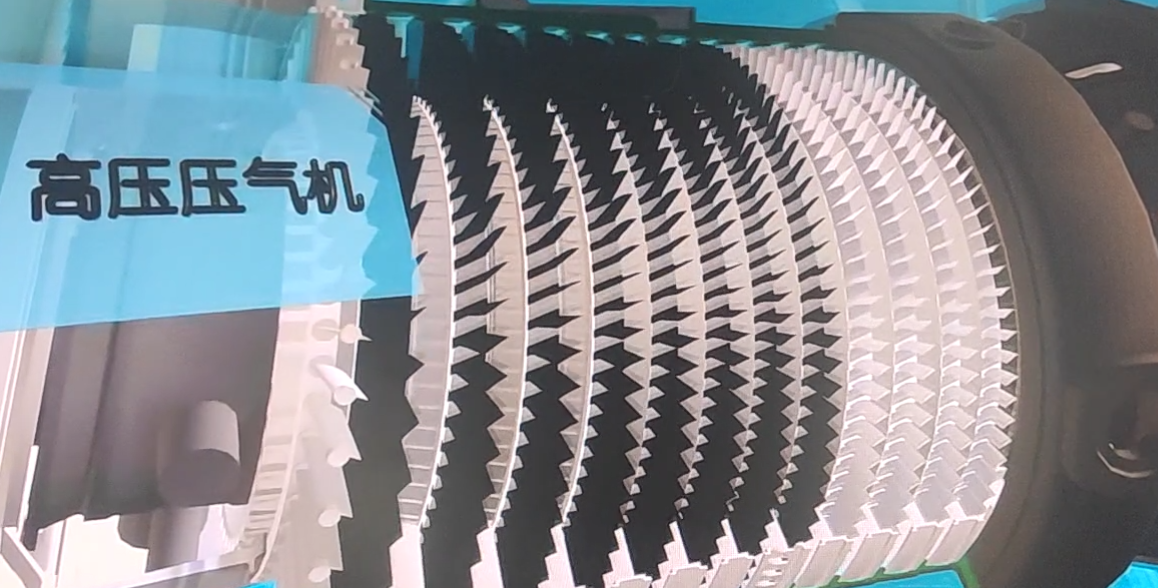
\includegraphics[width=0.85\textwidth]{figures/图3.png}
    \caption{发动机部件示意}
    \label{fig:engine_parts}
\end{figure}

\begin{figure}[H]
    \centering
    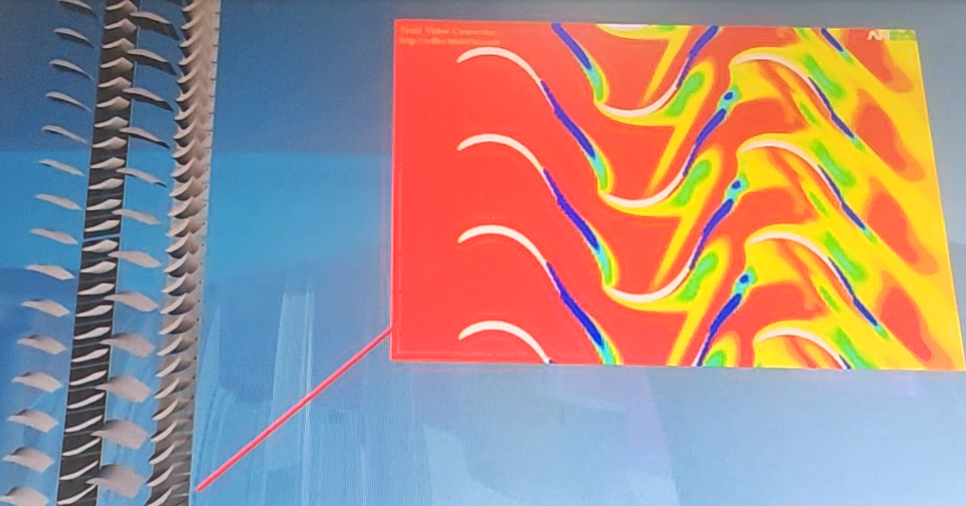
\includegraphics[width=0.90\textwidth]{figures/图9.png}
    \caption{涡轮叶栅流动——渐缩通道内的加速膨胀}
    \label{fig:turbine_flow}
\end{figure}

\textbf{通道几何与流动本质（图~\ref{fig:turbine_flow}）：} 该图展示了高压燃气通过涡轮叶栅时的加速膨胀过程。与压气机叶栅的"渐扩减速增压"通道截然相反，涡轮转子/静子叶片之间构成了明显的渐缩通道（Convergent Passage）。气流在巨大的落压比驱动下，静压能与热能剧烈转化为动能，槽道内的气流表现出极强的压降与加速度。

\textbf{流场云图物理特性：}

\textbf{能量转化梯度：} 图中大面积的红色背景以及向出口方向剧烈的颜色梯度变化，直观地反映了气流马赫数的激增（由低速亚音速膨胀至高亚音速甚至跨声速段），以及静压/静温在轴向上的骤降。

\textbf{局部高载荷区：} 在叶片吸力面的前中部，由于通道收缩和气流转折，气流膨胀速度达到峰值，形成局部的高马赫数区；而压力面相对平缓，这种两侧巨大的流速差形成了驱使涡轮旋转作功的叶片气动力。

\textbf{尾迹与落后角：} 在叶片后缘，可以清晰观察到由于边界层汇聚并脱落形成的狭窄尾迹损失区。若该级为跨声速涡轮，后缘还会伴随有复杂的膨胀波与内剪切激波系，这是阻碍涡轮效率进一步提升的关键流动损失来源。

\subsubsection{排气混合器与加力燃烧室流动观察}

\begin{figure}[H]
    \centering
    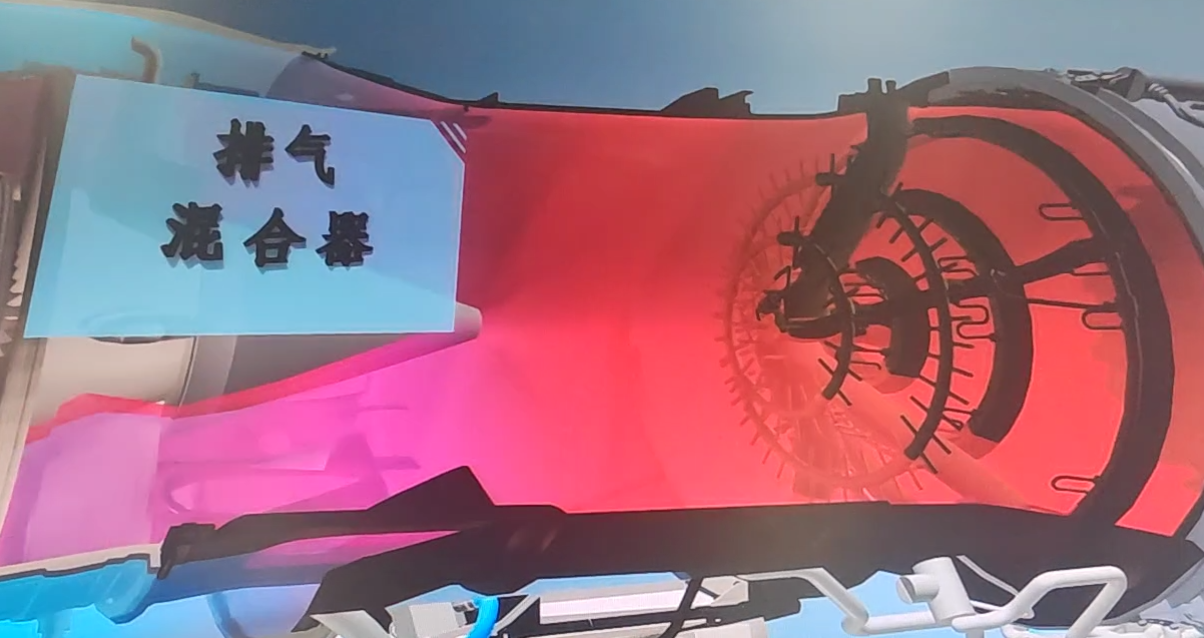
\includegraphics[width=0.90\textwidth]{figures/图10.png}
    \caption{波瓣形排气混合器——冷热气流掺混}
    \label{fig:mixer}
\end{figure}

\textbf{排气混合器（图~\ref{fig:mixer}）：} 展示了典型的波瓣形混合器（Lobed Mixer）结构。通过三维剖面可以观察到，核心机排出的高温燃气（红色区域）与外涵道排出的较低温冷空气在此汇合。波瓣结构极大地扩展了冷热气流的剪切接触面积，并利用几何形状诱导产生强大的流向涡（Streamwise vortices）。这种强迫掺混机制能够有效均匀排气温度场，提升整体推进效率，并显著降低发动机的红外特征和排气噪声。

\begin{figure}[H]
    \centering
    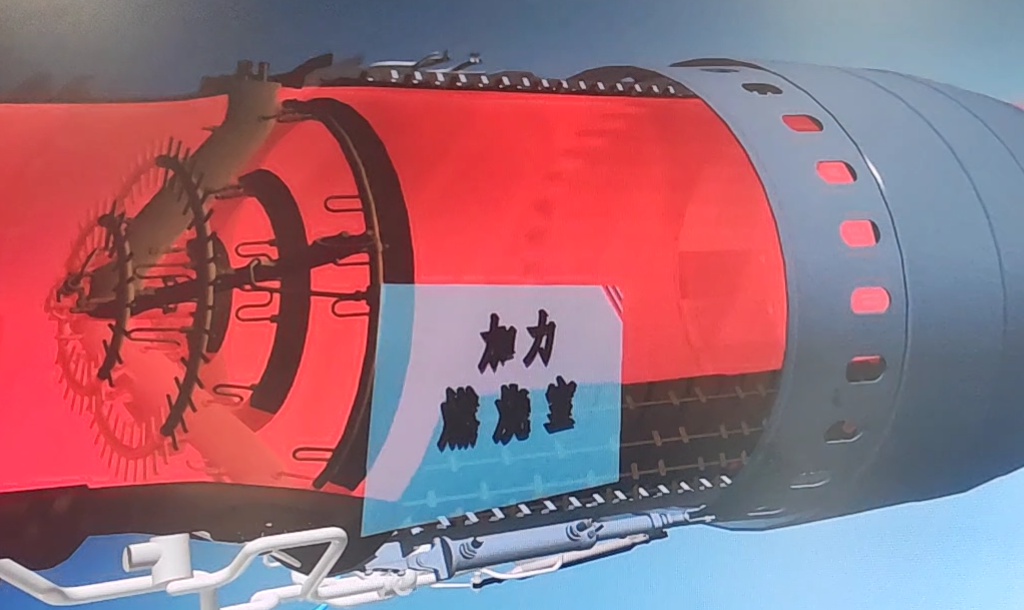
\includegraphics[width=0.90\textwidth]{figures/图11.png}
    \caption{加力燃烧室——火焰稳定器与尾流回流区}
    \label{fig:afterburner_flow}
\end{figure}

\textbf{加力燃烧室（图~\ref{fig:afterburner_flow}）：} 清晰展示了加力燃烧室内部的环形和径向火焰稳定器（V 型钝体/沙丘驻涡器，V-gutter）。在高速流动的排气环境中，气流流经这些非流线型的钝体时，会在其尾缘后方发生边界层分离，形成局部低速的尾流回流区。这一区域起到了"气动避风港"的作用，确保加力时喷入的燃油能够稳定着火，防止火焰被极高流速的主干气流吹熄（Blowout）。

\subsection{实验分析与讨论}

\begin{enumerate}
    \item \textbf{压气机正常流动与失速流动的对比}

    正常工况下，气流沿叶栅通道顺畅流动，附面层紧贴叶片表面，通道内逆压梯度连续均匀，实现了动能向压力能的有效转化。失速工况（如静叶关4°）下，叶片吸力面出现严重的附面层分离，分离区产生巨大的旋涡和回流，形成气动阻塞，通道增压能力丧失。这种由攻角异常增大诱发的分离是发动机喘振的直接原因。

    \item \textbf{燃烧室的稳焰机制与热管理}

    主燃区前段的双涡回流区由旋流器的强旋流作用产生，回流区将高温燃气带回火焰筒头部点燃新鲜混气，是火焰稳定的核心气动结构。温度云图显示截面中心温度梯度极大，壁面冷却气膜对保证火焰筒结构完整性至关重要。

    \item \textbf{排气混合器的波瓣结构}

    波瓣形混合器通过几何形状扩展冷热气流的剪切接触面积，诱导流向涡实现强迫掺混，均匀排气温度场，同时降低红外特征和排气噪声。

    \item \textbf{加力燃烧室的火焰稳定}

    V 型钝体/沙丘驻涡器在高速气流中产生尾流回流区，形成局部低速区使燃油稳定着火，防止被高速主流吹熄。
\end{enumerate}

\subsection{结论}

通过本次虚拟流动实验，结合 CFD 云图和流线可视化结果，对航空发动机四个关键部件的气动热力过程有了深入理解。压气机在设计攻角下流动顺畅而在异常攻角下发生附面层分离引发失速；燃烧室头部双涡回流区实现火焰稳定，壁面冷却气膜保证结构安全；波瓣混合器通过流向涡实现高效掺混；加力燃烧室 V 型钝体后方回流区防止火焰吹熄。实验加深了对《航空发动机原理》和《燃烧学》课程中相关内容的理解。
